\documentclass{jsarticle}
\usepackage[dvipdfmx]{hyperref}
\usepackage[dvipdfmx]{graphicx}
\usepackage{amssymb,amsmath,amsthm}
\usepackage{listings,jlisting}
\usepackage{newtxtt}
\usepackage[utf8]{inputenc}
\lstset{
  language=Python,      
  basicstyle={\small},%
  identifierstyle={\small},%
  commentstyle={\small\itshape},%
  keywordstyle={\small\bfseries},%
  ndkeywordstyle={\small},%
  stringstyle={\small\ttfamily},
  frame={tblr},
  breaklines=true,
  columns=[l]{fullflexible},%
% numbers=left,%
  xrightmargin=0zw,%
  xleftmargin=3zw,%
  numberstyle={\scriptsize},%
  stepnumber=1,
  numbersep=1zw,%
  lineskip=-0.5ex%
}
\newcommand{\kakko}[1][]{(#1)}
\newcommand{\bx}{\bold{x}}
\newcommand{\bb}{\bold{b}}
\newcommand{\bd}{\bold{d}}


\date{\today}
\author{山田龍}
\title{}
\begin{document}
\maketitle
\section{Gauss-Seidel法}
SOR法の導出を知りたかったので、ここに示した。
Gauss-Seidel法とSOR法の導出については\cite{suuchi}の導出を参考にしながら行間をできる限り埋めた。
\begin{equation}
    A = D + L + U
\end{equation}
の順番で対角成分、下三角成分、上三角成分を定義する。
解くべき連立方程式は、
\begin{align}
  (D + L + U)\bx = \bb  \\
  \bx = -D^{-1}(L + U)\bx +  D^{-1} \bb 
\end{align}
ヤコビ法では、以下の漸化式が成立すれば$x^{\kakko[k]}$は連立方程式の解である。
\begin{equation}
    \bx^{\kakko[k+1]} = - D^{-1} L \bx^{\kakko[k]}\\
    - D^{-1} U \bx^{\kakko[k]} + D^{-1}\bold{b} 
\end{equation}
Gauss-Seidel法では、以下の漸化式が成立すれば$x^{\kakko[k]}$は連立方程式の解である。
\begin{align}
    \bx^{\kakko[k+1]} &= - D^{-1} L \bx^{\kakko[k+1]}
    - D^{-1} U \bx^{\kakko[k]} + D^{-1}\bold{b}\\
    &=- D^{-1} (L + U) \bx^{\kakko[k]} + D^{-1}\bold{b} 
\end{align}
反復の計算は、
\begin{align*}
    (E + D^{-1}L)\bx^{\kakko[k+1]} = - D^{-1} U \bx^{\kakko[k]} + D^{-1}\bold{b}\\
    (D + L)D^{-1}\bx^{\kakko[k+1]} = - D^{-1} U \bx^{\kakko[k]} + D^{-1}\bold{b}\\
    \bx^{\kakko[k+1]} = - (D + L)^{-1}U \bx^{\kakko[k]} +(D + L)^{-1}\bold{b}\\
\end{align*}
ここで、$\bd^{\kakko[k+1]} = \bx^{\kakko[k+1]} - \bx^{\kakko[k]}$を定義する。
\begin{align*}
  \bd^{\kakko[k+1]} &= - \left[ (D + L)^{-1}U + E\right] \bx^{\kakko[k]} + (D + L)^{-1}\bb\\
  &= - \left[ (D + L)^{-1}U - D^{-1}U + D^{-1}U+ E\right] \bx^{\kakko[k]}\\
  &+ \left[(D + L)^{-1} - D^{-1} + D^{-1}\right]\bb\\
  &= - \left[ - L(D + L)^{-1}D^{-1}U + D^{-1}U+ E\right] \bx^{\kakko[k]}\\
  &+ \left[- L(D + L)^{-1}D^{-1}+ D^{-1}\right]\bb\\
  &= - D^{-1}L \bx^{\kakko[k+1]}- \left( D^{-1}U+ E\right) \bx^{\kakko[k]} + D^{-1}\bb
\end{align*}
更に変形する。
\begin{align*}
  (E + D^{-1}L)\bd^{\kakko[k+1]} \\ 
& = - D^{-1}L (- D^{-1} U \bx^{\kakko[k]} + D^{-1}\bold{b})\\
&- \left( D^{-1}U+ E\right) (- D^{-1} U \bx^{\kakko[k-1]} + D^{-1}\bold{b})\\
&+ (D^{-1} + D^{-1} L D^{-1}) \bb\\
&=  - D^{-1}L D^{-1} U \bx^{\kakko[k]} - D^{-1}L D^{-1}\bold{b}\\
&+ \left( D^{-1}UD^{-1} U+ D^{-1} U\right)  \bx^{\kakko[k-1]} \\
&-( D^{-1}UD^{-1} + D^{-1})\bold{b}\\
&+ (D^{-1} + D^{-1} L D^{-1})\bb
\end{align*}
両辺変形して、
\begin{align*}
D^{-1}(D + L)\bd^{\kakko[k+1]} &= D^{-1} [-L D^{-1} U \bx^{\kakko[k]} - L D^{-1}\bold{b}\\
&+ \left( UD^{-1} U+ U\right)  \bx^{\kakko[k-1]} \\
&+(-UD^{-1} + LD^{-1})\bold{b}]\\
(D + L)\bd^{\kakko[k+1]}&= - L D^{-1} U \bx^{\kakko[k]} - L D^{-1}\bold{b}\\
&+ \left( UD^{-1} U+ U\right)  \bx^{\kakko[k-1]} \\
& + (-UD^{-1} + LD^{-1})\bold{b}\\
\end{align*}
左辺の係数の逆行列を両辺にかけて、
\begin{align*}
\bd^{\kakko[k+1]} &= (D + L)^{-1}U[- L D^{-1}  \bx^{\kakko[k]} + \left( D^{-1} U+ E\right) \bx^{\kakko[k-1]}
-D^{-1}\bold{b}]\\
&= (D + L)^{-1}U\bd^{\kakko[k]}\\
\end{align*}
よってGauss-Seidel法において解が収束する条件は、
\begin{equation}
    ||(D + L)^{-1}U||_2 < 1
\end{equation}
反復すべき式は、
\begin{align}
    D\bx^{\kakko[k+1]} = - L\bx^{\kakko[k+1]} - U\bx^{\kakko[k]}+\bb\\
    a_{ii}\bx^{\kakko[k+1]}_i =
    - \sum^{i-1}_{j=1} a_{ij}\bx^{\kakko[k+1]}_j- \sum^{n}_{j=i+1}a_{ij}\bx^{\kakko[k+1]}_j+\bb_i
\end{align}
\section{SOR法}
Gauss-Seidel法において、緩和係数$\omega$を持ち込んで改良した解法をSOR法という。
Gauss-Seidel法の計算式を変形する。
\begin{align}
&    (E + D^{-1}L)\bx^{\kakko[k+1]} = - D^{-1} U \bx^{\kakko[k]} + D^{-1}\bold{b}\\
&    \bx^{\kakko[k+1]} = \bx^{\kakko[k]}-D^{-1}L\bx^{\kakko[k+1]}- (D^{-1} U+E) \bx^{\kakko[k]} + D^{-1}\bold{b}
\end{align}
SOR法では緩和係数$\omega$を導入する。
\begin{align}
  \bx^{\kakko[k+1]} = \bx^{\kakko[k]} +\omega\left[-D^{-1}L\bx^{\kakko[k+1]}- (D^{-1} U+E) \bx^{\kakko[k]} + D^{-1}\bb \right]\\
  (E + \omega D^{-1}L)\bx^{\kakko[k+1]} = \left[E-\omega(D^{-1} U+E)\right] \bx^{\kakko[k]} + \omega D^{-1}\bb 
\end{align}
反復すべき式は、
\begin{align}
  D\bx^{\kakko[k+1]} = D\bx^{\kakko[k]} +\omega\left[-L\bx^{\kakko[k+1]}- (U+D) \bx^{\kakko[k]} + \bb \right]\\
  D\bx^{\kakko[k+1]} = - \omega L\bx^{\kakko[k+1]} +\left[D- \omega (U+D)\right] \bx^{\kakko[k]} + \omega\bb 
\end{align}
成分表示すれば、
\begin{equation}
a_{ii}\bx^{\kakko[k+1]}_i = - \omega\sum^{i-1}_{j=1} a_{ij}\bx^{\kakko[k+1]}_j + (1- \omega) a_{ii}\bx^{\kakko[k]}_i -\omega\sum^{n}_{j=i+1}a_{ij}\bx^{\kakko[k]}_j+\omega\bb_i
\end{equation}
緩和係数は問題に応じて選択される。
\section{課題1}
\begin{equation}
  \left(
  \begin{array}{rrrr}
      10 & 1 & 4& 0\\
      1 & 10 & 5 & -1\\
      4 & 5 & 10 & 7\\
      0 & -1 & 7 & 9 
  \end{array}
  \right)
  \left(
  \begin{array}{r}
      x_1\\
      x_2\\
      x_3\\
      x_4 
  \end{array}
  \right)
  =
  \left(
  \begin{array}{r}
      15\\
      15\\
      26\\
      15
  \end{array}
  \right)
\end{equation}
\begin{equation}
  \left(
  \begin{array}{rrrr}
      10 & 1 & 4& 0\\
      1 & 10 & 5 & -1\\
      4 & 5 & 10 & 7\\
      0 & -1 & 7 & 9 
  \end{array}
  \right)
  \left(
  \begin{array}{r}
      x_1\\
      x_2\\
      x_3\\
      x_4 
  \end{array}
  \right)
  =
  \left(
  \begin{array}{r}
      16\\
      16\\
      25\\
      16
  \end{array}
  \right)
\end{equation}
の解をGaussの消去法を用いて求める。
\subsection{単精度と倍精度}
計算機において実数を表示するためには浮動小数点法が使われる。
計算機の内部において$2$進数が使われていたとき、
その表現は、以下のよう記述できる。
\begin{equation}
  \pm (1.a_1 a_2 \cdots a_m) \times 2^e
\end{equation}
では、単精度の場合に指数部が$8$ビットであったとしよう。
いま、$10$進数で$12.5$の数値を浮動小数点表示したいとする。
まず符号は$+$なので符号の部分のビットは$0$である。
$12.5$は$2$進数表示で$1.1001 \times 2^3$と表される。
指数部分はバイアス$128-1=127$を使った記法を用いれば、$(3 + 127)_{10} =(130)_{10} = (10000010)_2$となる。
仮数部は、正規化された$2$進数表示の場合には必ず先頭は$1$になるので、先頭を省略して
$10010\cdots0$となる。図示すれば以下のようになる。


\begin{tabular}{|c|c|c|c|c|c|c|c|c|c|c|c|c|c|c|c|c|}\hline
1&2&3&4&5&6&7&8&9&10&11&12&13&14&15&$\cdots$&32\\\hline
符号 & 指数部&-&-&-&-&-&-&-&仮数部&-&-&-&-&-&$\cdots$&-\\\hline
0&1&0&0&0&0&0&1&0&1&0&0&1&0&0&$\cdots$&0\\\hline
\end{tabular}



numpyのfloat32、float64においては、numpy.finfo関数を使ってそれぞれの仕様を確認することができる。

\begin{lstlisting}
  Machine parameters for float32
precision =   6   resolution = 1.0000000e-06
machep =    -23   eps =        1.1920929e-07
negep =     -24   epsneg =     5.9604645e-08
minexp =   -126   tiny =       1.1754944e-38
maxexp =    128   max =        3.4028235e+38
nexp =        8   min =        -max
\end{lstlisting}
\begin{lstlisting}
  Machine parameters for float64
precision =  15   resolution = 1.0000000000000001e-15
machep =    -52   eps =        2.2204460492503131e-16
negep =     -53   epsneg =     1.1102230246251565e-16
minexp =  -1022   tiny =       2.2250738585072014e-308
maxexp =   1024   max =        1.7976931348623157e+308
nexp =       11   min =        -max
\end{lstlisting}

ここから、単精度では指数部が$8bit$で仮数部が$32-1-8=23bit$あるので$10$進数では6桁の精度、
倍精度では指数部が$11bit$で仮数部が$64-1-11=52bit$あるので$10$進数では15桁の精度があることがわかる。
\subsection{$b=(15, 15, 26, 15)^T$の場合}
Gaussの消去法を使って$A\bx = \bb$の解$\bx$を求めた。
単精度では、
\begin{lstlisting}
  x: [1.        1.0000001 0.9999999 1.       ]
  A * x: [14.99999964 15.0000006  25.9999994  14.99999905]
\end{lstlisting}
倍精度では、
\begin{lstlisting}
  x: [1. 1. 1. 1.]
  A * x: [15. 15. 26. 15.]
\end{lstlisting}
比較すると、単精度の場合には$7$桁目以降で誤差が生じている。

\subsection{$b=(16, 16, 25, 16)^T$の場合}
Gaussの消去法を使って$A\bx = \bb$の解$\bx$を求めた。
単精度では、
\begin{lstlisting}
  x: [  832.18555  1324.2953  -2407.5376   2021.451  ]
  A * x: [16.00036621 15.99938965 25.         16.00097656]
\end{lstlisting}
倍精度では、
\begin{lstlisting}
  x: [  832.  1324. -2407.  2021.]
  A * x: [16. 16. 25. 16.]
\end{lstlisting}
比較すると、$4$桁目以降に誤差が生じており、単精度の範囲での演算では誤差が大きくなっている。
\section{課題2}
\begin{equation}
  \left(
  \begin{array}{rrrr}
      1 & -1 & 0& 0\\
      -1 & 2 & -1 & 0\\
      0 & -1 & 0 & -1\\
      0 & 0 & -1 & 2 
  \end{array}
  \right)
  \left(
  \begin{array}{r}
      x_1\\
      x_2\\
      x_3\\
      x_4 
  \end{array}
  \right)
  =
  \left(
  \begin{array}{r}
      1\\
      0\\
      0\\
      0
  \end{array}
  \right)
\end{equation}
の解をSOR法を用いて求める。

\subsection{解と反復係数}
解を計算によって求めた。
\begin{lstlisting}
  x: [ 0.72727273 -0.27272727 -0.18181818 -0.09090909]
\end{lstlisting}
横軸を反復回数、縦軸を真の解からの誤差のノルムの対数にとる。また、計算は$10$桁よりも発散が大きくなったら打ち切る。
この条件のもとで、$\omega$の値を変えてプロットすると以下のようになる。
\begin{figure}[htbp]
    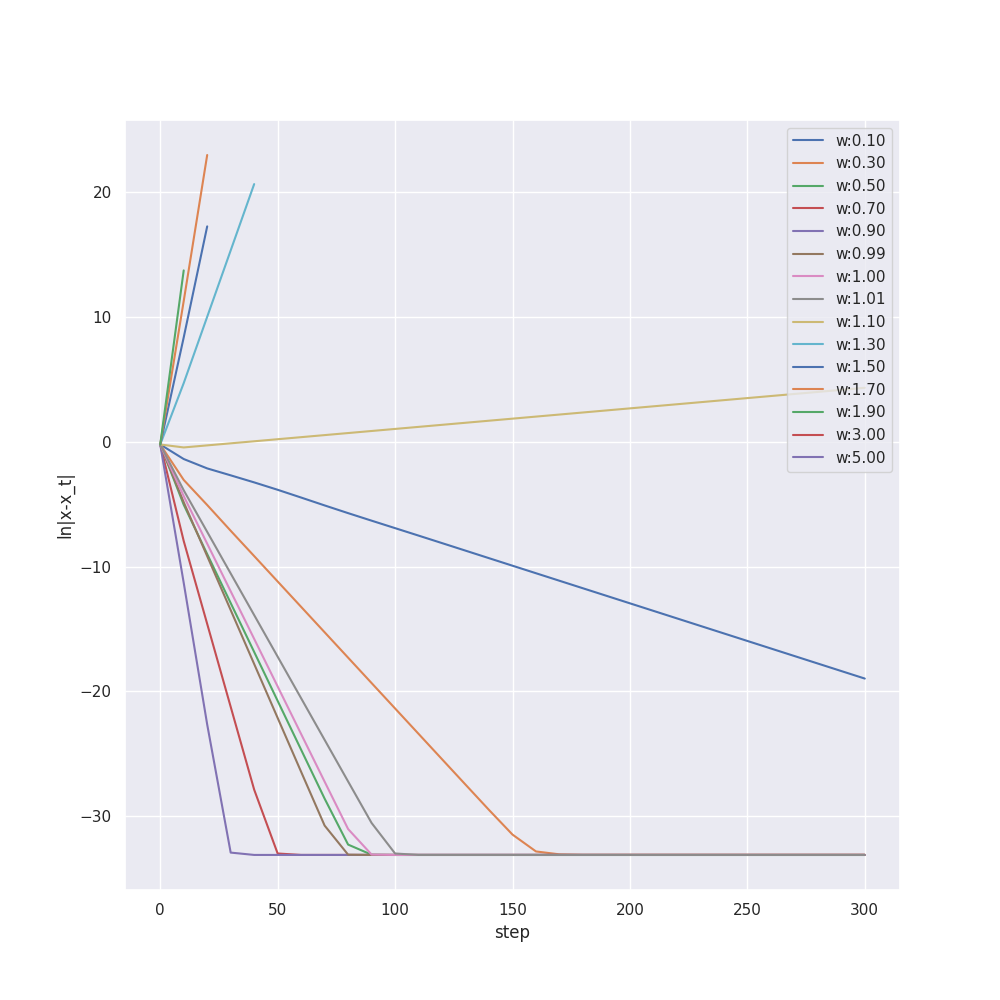
\includegraphics[clip,width=15.0cm]{./sor.png}
    \caption{SOR法の誤差}
\end{figure}
$w<=1$では収束、$w>1$では発散している。
プログラムのミスによるものかを確認するために、例えば、課題$1$で指定されたような連立方程式に対してSOR法を用いると、以下のようになる。
\begin{figure}[htbp]
    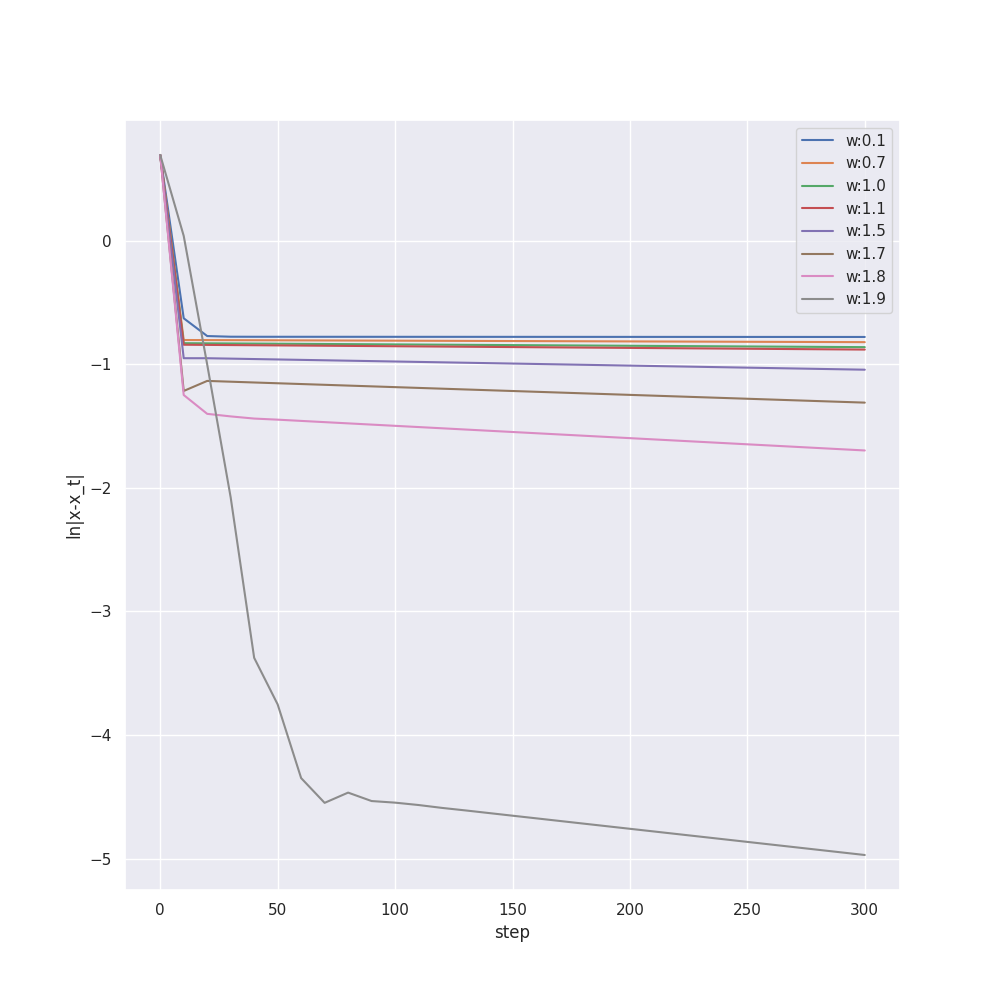
\includegraphics[clip,width=15.0cm]{./sor_debug.png}
    \caption{SOR法の誤差}
\end{figure}


すべての$0<\omega<2$の緩和係数に対して収束している。
また、$\omega = 1.9$のときだけ精度が他の緩和係数のときよりも高いこともわかった。

プログラムは正しく走っていると考えられるので、最初の場合に$\omega$が$1$よりも少し高いところから先で発散している理由を考えた。
私は、行列の固有値が$3,	2.2469796037175,	-0.80193773580484,	0.55495813208737$で絶対値が$1$より大きいものがあることから、
本当はGauss-Seidel法が使えない状況であるために$w$が$1$より小さい場合にのみ収束したと考えた。

\section{プログラム}
ソースコードを添付しますが、全て
\href{https://github.com/tychy/NumericalAnalysisPlayground}{https://github.com/tychy/NumericalAnalysisPlayground}にあります。
各関数のテストもついています。
\begin{lstlisting}[caption=gaussの消去法,label=参照ラベル]
import numpy as np


def scale(A, x):
    scale_ls = np.zeros_like(x)
    for i in range(A.shape[0]):
        max_idx = 0
        for j in range(A.shape[0]):
            if np.abs(A[i, j]) > np.abs(A[i, max_idx]):
                max_idx = j
        scale_ls[i] = np.abs(A[i, max_idx])
        x[i] = x[i] / np.abs(A[i, max_idx])
        A[i, :] = A[i, :] / np.abs(A[i, max_idx])
    return scale_ls


def pivot(A, x, idx):
    max_idx = idx
    for i in range(idx, A.shape[0]):
        if A[idx, i] > A[idx, max_idx]:
            max_idx = i
    if max_idx != idx:
        buff = np.copy(A[max_idx, :])
        A[max_idx, :] = A[idx, :]
        A[idx, :] = buff
        buffx = x[max_idx]
        x[max_idx] = x[idx]
        x[idx] = buffx
    return


def execute(A, b):
    assert A.shape[0] == A.shape[1], "A must be n * n"
    assert A.shape[0] == b.shape[0], "size of A and b must match"
    print("A:", A)
    print("b:", b)
    L = np.zeros_like(A)
    for i in range(A.shape[0]):
        L[i, i] = 1
    scale_ls = scale(A, b)
    print("Scaled A:", A)

    pivot(A, b, 0)
    for i in range(1, A.shape[0]):
        pivot(A, b, i)
        for j in range(i, A.shape[0]):
            coef = A[j][i - 1] / A[i - 1][i - 1]
            A[j, :] = A[j, :] - A[i - 1, :] * coef
            b[j] = b[j] - b[i - 1] * coef
            L[j, i - 1] = coef
    x = np.zeros_like(b)
    print("L:", L)
    for i in range(A.shape[0] - 1, -1, -1):
        x[i] += b[i]
        for j in range(i, A.shape[0] - 1):
            x[i] -= A[i][j + 1] * x[j + 1]
        x[i] /= A[i][i]
    print("x:", x)
    for i in range(A.shape[0]):
        A[i, :] = A[i, :] * scale_ls[i]

    return x, L, A


def single(A, b):
    print("-----single-----")
    A_copy = np.copy(A).astype(np.float32)
    b_copy = np.copy(b).astype(np.float32)
    fi32 = np.finfo(np.float32)
    print(fi32)
    x, L, U = execute(A_copy, b_copy)
    print("A * x:", A @ x.T)
    print("-----END-----")


def double(A, b):
    print("double")

    A_copy = np.copy(A).astype(np.float64)
    b_copy = np.copy(b).astype(np.float64)
    fi64 = np.finfo(np.float64)
    print(fi64)
    x, L, U = execute(A_copy, b_copy)
    print("A * x:", A @ x.T)
    print("-----END-----")


if __name__ == "__main__":
    A = np.array(
        [
            [10.0, 1.0, 4.0, 0.0],
            [1.0, 10.0, 5.0, -1.0],
            [4.0, 5.0, 10.0, 7.0],
            [0.0, -1.0, 7.0, 9.0],
        ],
    )
    b = np.array([15.0, 15.0, 26.0, 15.0])
    c = np.array([16.0, 16.0, 25.0, 16.0])

    single(A, b)
    double(A, b)
    single(A, c)
    double(A, c)

\end{lstlisting}
\begin{lstlisting}[caption=SOR法,label=参照ラベル]
import numpy as np
import matplotlib.pyplot as plt
import seaborn as sns


def split_matrix(A):
    D = np.zeros_like(A)
    L = np.zeros_like(A)
    U = np.zeros_like(A)
    for i in range(A.shape[0]):
        D[i, i] = A[i, i]

    for i in range(A.shape[0]):
        for j in range(i):
            L[i, j] = A[i, j]

    for i in range(A.shape[0]):
        for j in range(i + 1, A.shape[0]):
            U[i, j] = A[i, j]
    print("D:", D)
    print("L:", L)
    print("U:", U)
    return D, L, U


def execute(A, b, w, x_true):
    assert A.shape[0] == A.shape[1], "A must be n * n"
    assert A.shape[0] == b.shape[0], "size of A and b must match"
    print("A:", A)
    print("b:", b)
    # D, L, U = split_matrix(A)
    x_prev = np.zeros_like(b)
    x = np.zeros_like(b)
    step_ls = []
    x_ls = []
    step = 0
    max_step = 300
    while step <= max_step:
        if np.linalg.norm(x - x_true) > np.power(10, 10):
            break
        if step % 10 == 0:
            step_ls.append(step)
            x_ls.append(np.log(np.linalg.norm(x - x_true)))
        x_prev = np.copy(x)
        for i in range(A.shape[0]):
            mida = 0
            midb = 0
            for j in range(i):
                mida += A[i, j] * x[j]
            for j in range(i + 1, A.shape[0]):
                midb += A[i, j] * x_prev[j]
            x[i] = (
                -w * mida + (1 - w) * A[i, i] * x_prev[i] - w * midb + w * b[i]
            ) / A[i, i]
        step += 1
    print("x:", x)
    return x, step_ls, x_ls


def double(A, b, w, x_true):
    print("-----double-----")
    print("omega:", w)
    A_copy = np.copy(A).astype(np.float64)
    b_copy = np.copy(b).astype(np.float64)
    x, step_ls, x_ls = execute(A_copy, b_copy, w, x_true)
    print("A * x:", A @ x.T)
    print("-----END-----")
    return step_ls, x_ls


def plot_sor():
    sns.set_theme()
    A = np.array(
        [
            [1.0, -1.0, 0.0, 0.0],
            [-1.0, -2.0, -1.0, 0.0],
            [0.0, -1.0, 2.0, -1.0],
            [0.0, 0.0, -1.0, 2.0],
        ],
    )
    b = np.array([1.0, 0.0, 0.0, 0.0])
    x_true = np.array(
        [0.72727272727273, -0.27272727272727, -0.18181818181818, -0.090909090909091]
    )
    fig = plt.figure(figsize=(10, 10))
    for w in [0.1, 0.3, 0.5, 0.7, 0.9, 0.99, 1.0, 1.01, 1.1, 1.3, 1.5, 1.7, 1.9, 3, 5]:
        step_ls, x_ls = double(A, b, w, x_true)
        plt.plot(step_ls, x_ls, label="w:{:.2f}".format(w))

    plt.xlabel("step")
    plt.ylabel("ln|x-x_t|")
    plt.legend()
    plt.savefig("sor.png")


def plot_sor_debug():
    sns.set_theme()
    A = np.array(
        [
            [10.0, 1.0, 4.0, 0.0],
            [1.0, 10.0, 5.0, -1.0],
            [4.0, 5.0, 10.0, 7.0],
            [0.0, -1.0, 7.0, 9.0],
        ],
    )
    b = np.array([15.0, 15.0, 26.0, 15.0])

    x_true = np.array([1, 1, 1, 1])
    fig = plt.figure(figsize=(10, 10))

    for w in [0.1, 0.7, 1.0, 1.1, 1.5, 1.7, 1.8, 1.9]:
        step_ls, x_ls = double(A, b, w, x_true)
        plt.plot(step_ls, x_ls, label="w:{:.1f}".format(w))

    plt.xlabel("step")
    plt.ylabel("ln|x-x_t|")
    plt.legend()
    plt.savefig("sor_debug.png")


if __name__ == "__main__":
    plot_sor()
    plot_sor_debug()
\end{lstlisting}
\bibliographystyle{junsrt}
\bibliography{cite}
\end{document}